\documentclass{llncs}
%\documentclass{article}

\usepackage{graphicx,array}
\usepackage{amsmath}
\usepackage{amssymb}
\usepackage{amsfonts}
\usepackage{epsfig}
\usepackage{float}
%\usepackage{supertabular} % used in B Symbols


%% Keywords for the B method
\newcommand{\MACHINE}{\operatorname{\mathbf{MACHINE}}}
\newcommand{\REFINEMENT}{\operatorname{\mathbf{REFINEMENT}}}
\newcommand{\IMPLEMENTATION}{\operatorname{\mathbf{IMPLEMENTATION}}}
\newcommand{\REFINES}{\operatorname{\mathbf{REFINES}}}
\newcommand{\SEES}{\operatorname{\mathbf{SEES}}}
\newcommand{\INCLUDES}{\operatorname{\mathbf{INCLUDES}}}
\newcommand{\IMPORTS}{\operatorname{\mathbf{IMPORTS}}}
\newcommand{\SETS}{\operatorname{\mathbf{SETS}}}
\newcommand{\CONSTANTS}{\operatorname{\mathbf{CONSTANTS}}}
\newcommand{\PROPERTIES}{\operatorname{\mathbf{PROPERTIES}}}
\newcommand{\CONCRETE}{\operatorname{\mathbf{CONCRETE}}}
\newcommand{\VARIABLES}{\operatorname{\mathbf{VARIABLES}}}
\newcommand{\ASSERTIONS}{\operatorname{\mathbf{ASSERTIONS}}}
\newcommand{\CONCRETEVARIABLES}{\operatorname{\mathbf{CONCRETE\_VARIABLES}}}
\newcommand{\DEFINITIONS}{\operatorname{\mathbf{DEFINITIONS}}}
\newcommand{\VAR}{\operatorname{\mathbf{VAR}}}
\newcommand{\IN}{\operatorname{\mathbf{IN}}}
\newcommand{\INVARIANT}{\operatorname{\mathbf{INVARIANT}}}
\newcommand{\INITIALISATION}{\operatorname{\mathbf{INITIALISATION}}}
\newcommand{\OPERATIONS}{\operatorname{\mathbf{OPERATIONS}}}
\newcommand{\BEGIN}{\operatorname{\mathbf{BEGIN}}}
\newcommand{\END}{\operatorname{\mathbf{END}}}
\newcommand{\PRE}{\operatorname{\mathbf{PRE}}}
\newcommand{\IF}{\operatorname{\mathbf{IF}}}
\newcommand{\THEN}{\operatorname{\mathbf{THEN}}}
\newcommand{\ELSE}{\operatorname{\mathbf{ELSE}}}
\newcommand{\ELSIF}{\operatorname{\mathbf{ELSIF}}}
\newcommand{\ANY}{\operatorname{\mathbf{ANY}}}
\newcommand{\WHERE}{\operatorname{\mathbf{WHERE}}}
\newcommand{\CASE}{\operatorname{\mathbf{CASE}}}
\newcommand{\OF}{\operatorname{\mathbf{OF}}}
\newcommand{\EITHER}{\operatorname{\mathbf{EITHER}}}
\newcommand{\AND}{\operatorname{\mathbf{AND}}}
\newcommand{\OR}{\operatorname{\mathbf{OR}}}
\newcommand{\NOT}{\operatorname{\mathbf{NOT}}}
\newcommand{\WHILE}{\operatorname{\mathbf{WHILE}}}
\newcommand{\DO}{\operatorname{\mathbf{DO}}}
\newcommand{\VARIANT}{\operatorname{\mathbf{VARIANT}}}
\newcommand{\FALSE}{\operatorname{\mathbf{FALSE}}}
\newcommand{\TRUE}{\operatorname{\mathbf{TRUE}}}

%% Commonly used math entities
\newcommand{\pow}{\operatorname{\mathbb{P}}}
\newcommand{\nat}{\operatorname{\mathbb{N}}}
\newcommand{\pfun}{\operatorname{\rightarrow\mkern-22mu+}}
\newcommand{\fset}{\operatorname{\mathbb{F}}}
\newcommand{\dom}{\operatorname{\mbox{dom}}}
\newcommand{\ran}{\operatorname{\mbox{ran}}}
\newcommand{\natone}{\operatorname{\mathbb{N}_1}}
\newcommand{\integer}{\operatorname{\mathbb{Z}}}
\newcommand{\fun}{\operatorname{\rightarrow}}
\newcommand{\domr}{\operatorname{\triangleleft}}
\newcommand{\seq}{\operatorname{\mathbf{seq1}}}
\newcommand{\ovr}{\operatorname{\oplus}}
\newcommand{\BOOL}{\operatorname{\mathbf{BOOL}}}
\newcommand{\pred}{\operatorname{\mathbf{pred}}}
\newcommand{\Bsucc}{\operatorname{\mathbf{succ}}}


%\usepackage{supertabular}

% DEFINITION DES CARACTERES MATHEMATIQUES B
%------------------------------------------
\def\@setmcodes#1#2#3{{\count0=#1 \count1=#3
	\loop \global\mathcode\count0=\count1 \ifnum \count0<#2
	\advance\count0 by1 \advance\count1 by1 \repeat}}

%\@setmcodes{`A}{`Z}{"7441}
%\@setmcodes{`a}{`z}{"7461}

\mathcode`\;="8000 % Makes ; active in math mode
{\catcode`\;=\active \gdef;{\semicolon\;}}
\mathchardef\semicolon="003B
%    Nominal distance from top of paper to top of page
% \topmargin 0 pt
% \textheight 53\baselineskip
% 
% %   Left margin on odd-numbered pages
% \oddsidemargin  0.15 in
% %   Left margin on even-numbered pages
% \evensidemargin 0.35 in
% %   Width of marginal notes.
% \marginparwidth 1 in
% %   Note that \oddsidemargin = \evensidemargin
% \oddsidemargin 0.25 in
% \evensidemargin 0.25 in
% \marginparwidth 0.75 in
% \textwidth 5.875 in % Width of text line.
% 
% \setlength{\parindent}{0pt}
% \setlength{\parskip}{0ex}

% DEFINITION DES FONTS
%---------------------
% The AMS extra symbol fonts are loaded.
% Note: sometimes called euxm10
\font\msx=msam10
% Note: sometimes called euym10
\font\msy=msbm10

\newfam\msxfam \textfont\msxfam=\msx
\newfam\msyfam \textfont\msyfam=\msy

\def\famletter#1{\ifcase #1 0\or 1\or 2\or 3\or 4\or 5\or 6\or 7\or
	8\or 9\or A\or B\or C\or D\or E\or F\fi}

\edef\fx{\famletter\msxfam}
\edef\fy{\famletter\msyfam}

\def\bbold{\fam\msyfam \msy}

% SYMBOLES B
%-----------
% makes a quoted expression in mathematical text
\def\token#1{\hbox{`$#1$'}}
% used for error messages in Z specs
\def\report#1{\hbox{`{\tt #1}'}}

% \@myop makes an operator, with a strut to defeat TeX's vertical adjustment.
\def\@myop#1{\mathop{\mathstrut{#1}}\nolimits}

% This underscore doesn't have the little kern --- you get an italic
% correction anyway in math mode.
\def\_{\leavevmode \vbox{\hrule width0.5em}}

% Save \q as \xq for quantifiers q.
\let\xforall=\forall
\let\xexists=\exists
\let\xlambda=\lambda
\let\xmu=\mu

% \p and \f make arrows with 1 and 2 crossings resp.
\def\p#1{\mathrel{\ooalign{\hfil$\mapstochar\mkern 5mu$\hfil\cr$#1$}}}
\def\f#1{\mathrel{\ooalign{\hfil
	$\mapstochar\mkern 3mu\mapstochar\mkern 5mu$\hfil\cr$#1$}}}

\let\mc=\mathchardef

\def	\pow		{\mbox{${\cal P}$}}
\def	\po1		{\mbox{${\cal P}_1$}}
\let	\cross		\times
\def	\lambda		{\@myop{\xlambda}}
\def	\lnot		{\neg\;}
\def	\land		{\mathrel{\wedge}}
\def	\lor		{\mathrel{\vee}}
\let	\implies	\Rightarrow
\let	\iff		\Leftrightarrow
\def	\forall		{\@myop{\xforall}}
\def	\exists		{\@myop{\xexists}}
\def	\semi		{\mathrel{\comp}}
\def	\ssemi		{\mathbin{\rm ;}}
\let	\ensembleVide	\emptyset
\let	\rel		\leftrightarrow
\def	\dom		{\@myop{\sf dom}}
\def	\ran		{\@myop{\sf ran}}
\def	\id		{\@myop{\sf id}}
\def	\comp		{\mathbin{\raise
			0.6ex\hbox{\oalign{\hfil$\scriptscriptstyle
			\rm o$\hfil\cr\hfil$\scriptscriptstyle\rm 9$\hfil}}}}
\def	\para		{\mbox{$\mid\mid$}}
\mc	\dres		"2\fx43
\mc	\rres		"2\fx42
\def	\ndres		{\mathbin{{\dres} \llap{$-$}}}
\def	\nrres		{\mathbin{{\rres}\llap{$-$}}}
\def	\lover		{\vartriangleleft{ \llap{$-\!\!\!\!-\!$}}}
\def	\rover		{\mathbin{{\rres}\llap{$\!-\!\!\!-$}}}
\let	\fun		\rightarrow
\def	\pfun		{\p\fun}
\def	\pinj		{\p\inj}
\mc	\inj		"3\fx1A
\def	\psurj		{\p\surj}
\mc	\surj		"3\fx10
\def	\bij		{\surj\!\!\!\!\!\!\!\inj}
\def	\nat		{\mbox{${\cal N}$}}
\def	\na1		{\mbox{${\cal N}_1$}}
\def	\num		{\mbox{${\cal Z}$}}
\def	\int		{\mbox{${\cal Z}$}}
\def	\rat		{\mbox{${\cal Q}$}}
\def	\div		{\mathbin{\rm /}}
\def	\mod		{\mathbin{\bf mod}}
\def	\upto		{\mathbin{\ldotp\ldotp}}
\def	\finset		{\mbox{${\cal F}$}}
\def	\finse1		{\mbox{${\cal F}_1$}}
\def	\ffun		{\f\fun}
\def	\finj		{\f\inj}
\def	\seq		{\@myop{\rm seq}}
\def	\cat		{\mathbin{\raise 0.8ex\hbox{$\mathchar"2\fx61$}}}
\def	\sep		{\hspace*{.05in}}

\setcounter{secnumdepth}{0}
\setcounter{tocdepth}{0}

%-------------------%
% Debut du document %
%-------------------%



 



%
\begin{document}

\title{Formal Construction of Microcontroller Instruction Set Model Using B}

\hyphenation{se-pa-ra-te}

\author{ David D\'{e}harbe\inst{1}, Val\'{e}rio Medeiros Jr\inst{2} }
\institute{Federal University of Rio Grande do Norte, Natal RN 59078-970, Brazil\inst{1} and\\  
Federal Institute of Education, Science and Technology of Rio Grande do Norte, Natal RN
59015-000, Brazil\inst{2}}


\maketitle

\begin{abstract}
  [To redo]
  This paper describes an approach to model the functional aspects of
  the instruction set of microcontroller platforms using the notation
  of the B method. The paper presents specifically the case of the Z80 
  platform. This work is a contribution towards the extension of the
  B method to handle developments up to assembly level code.
\end{abstract}
%
%\keywords{Fomal Methods, microcontroller Verification, Hardware}

\section{Introduction}
[To update]
The B method~\cite{Abrial} supports the construction of safety systems
models by verification of proofs that guarantees its correctness. So,
an initial abstract model of the system requirements is defined and
then it is refined until the implementation model. Development
environments based on the B method also include source code generators
for programming languages, but the result of this translation
cannot be compared by formal means. The paper \cite{Dantas_SBMF08} presented
recently an approach to extend the scope of the B method up to the
assembly level language. One key component of this approach
is to build, within the framework of the B method, formal models of
the instruction set of such assembly languages.

This work gives an overview of the formal modelling of the instruction
set of the Z80 microcontroller~\cite{Z80_manual}\footnote{The
  interested reader in more details is invited to visit our repository
  at: http://code.google.com/p/b2asm.}. Using the responsibility
division mechanism provided by B, auxiliary libraries of basic modules
were developed as part of the construction of microcontroller
model. Such library has many definitions about common concepts used in
the microcontrollers; besides the Z80 model, it is used by two other
microcontrollers models that are under way.

Other possible uses of a formal model of a microcontroller
instruction set include documentation, the construction of simulators,
and be possibly the starting point of a verification effort for the
actual implementation of a Z80 design. Moreover the model of the
instruction set could be instrumented with non-functional aspects,
such as the number of cycles it takes to execute an instruction, to
prove lower and upper bounds on the execution time of a routine. The
goal of this project, though, is to provide a basis for the generation
of software artifacts at the assembly level that are amenable to 
refinement verification within the B method.

This paper is focused on the presentation of the Z80 model, including
elementary libraries to describe hardware aspects. The paper is
structured as follows. Section~\ref{sec:B_method} provides a short
introduction to the B method. Section~\ref{sec:models} presents the
elementary libraries and the modelling of some elements common to
microcontrollers.  Section~\ref{sec:z80} presents the B model of the
Z80 instruction set. Section ~\ref{sec:Proofs} provides some
information on the proof effort needed to analyze the presented
models. Related work is discussed in
Section~\ref{sec:relatedworks}. Finally, the last section is devoted
to the conclusions.

\section{Introduction to the B Method}
\label{sec:B_method}

The B method for software development~\cite{Abrial} is based on the B Abstract
Machine Notation (AMN) and the use of formally proved refinements up to a
specification sufficiently concrete that programming code can be automatically
generated from it. Its mathematical basis consists of first order logic, integer
arithmetic and set theory, and its corresponding constructs are similar to those
of the Z notation.


A B specification is structured in modules. A module defines a set of valid
states, including a set of initial states, and operations that may provoke a
transition between states. The design process starts with a module with a
so-called functional model of the system under development. In this initial
modelling stage, the B method requires that the user proves that, in a machine,
all the its initial states are valid, and that operations do not define
transitions from valid states to invalid states.
  
Essentially, a B module contains two main parts: a header and the available
operations. Figure~\ref{fig:maqB} has a very basic example. The clause
$\mathit{MACHINE}$ has the name of module.  The next two clauses respectively
reference external modules and create an instance of an external module. The
$\mathit{VARIABLES}$ clauses declares the name of the variables that compose the
state of the machine. Next, the $\mathit{INVARIANT}$ clause defines the type and
other restrictions on the variables. The $\mathit{INITIALIZATION} $ specifies
the initial states. Finally, operations correspond to the transitions between
states of the machine.


\begin{figure}
  % \begin{small}
  $$
  \begin{array}{lcl}
    \begin{array}[t]{l}
      \MACHINE \quad  \mathit{micro} \\
      \SEES \quad \mathit{TYPES}, \mathit{ALU} \\
      \INCLUDES  \quad \mathit{MEMORY} \\
      \VARIABLES \quad    \mathit{pc}  \\
      \INVARIANT \quad \mathit{pc} \in \mathit{INSTRUCTION} 
    \end{array}
    & \hspace*{1cm} &
    \begin{array}[t]{l}
      \INITIALISATION  \mathit{pc} := 0 \\
      \OPERATIONS\\
      \mathit{JMP} \mathit{( jump )} = \\
      \quad \PRE \mathit{jump} \in \mathit{INSTRUCTION}\\ 
      \quad \THEN \mathit{pc} := \mathit{jump}\\  
      \quad \END \\
      \END
    \end{array}
  \end{array}
  $$
\caption{A very basic B machine.}
\label{fig:maqB}
\end{figure}


\section{Model structure and basic components}
\label{sec:models}

We have been developed a reusable set of basic definitions to model hardware concepts and data types
concepts. These definitions are grouped into two separate development projects and are available as
libraries. A third project is devoted to the higher-level aspects of the platform. Thus, the workspace is
composed of: a power library\footnote{The power library has the basics definitions to help the theorems
prover about simple calculus of power, especially power of two. It has constants, that represents all
results of power function needed, and the definition of power function.}, a hardware library, a types
library and a project for the specific platform, in this case the Z80. The corresponding dependency
diagram is depicted in Figure~\ref{fig:hardware-definition-graph}; information specific to each project is
presented in the following.


\begin{figure}[h] \centering
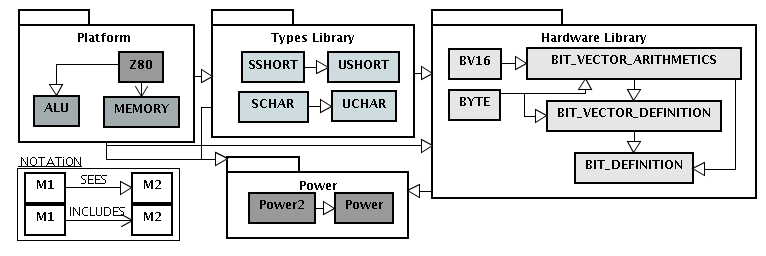
\includegraphics[width=.92\textwidth]{diagramaEstrutural_vertical.png}
 \caption{Dependency diagram of the Z80 model.}
\label{fig:hardware-definition-graph}
\end{figure}



\subsection{Bit Representation and Manipulation}

The entities defined in the module $\mathit{BIT\_DEFINITION}$ are the
type for bits, logical operations on bits (negation, conjunction,
disjunction, exclusive disjunction), as well as a conversion function
from booleans to bits.

First, bits are modelled as a set of integers: $\mathit{BIT} =
\mathit{0..1}$. The negation is an unary function on bits and it is
defined as:

$
\begin{array}{l}
\mathit{bit\_not}  \in  \mathit{BIT}  \fun  \mathit{BIT}  \land \forall ( \mathit{bb}). (\mathit{bb} \in \mathit{BIT} \implies \mathit{bit\_not}(\mathit{bb}) =
1-\mathit{bb})\\
\end{array}
$

The module also provides lemmas on negation that may be useful for the
users of the library to develop proofs:

$
\begin{array}{l}
%  \mathit{bit\_not}(0) = 1;  \mathit{bit\_not}(1) = 0; \\
\forall (\mathit{bb}).(\mathit{bb} \in \mathit{BIT} \implies \mathit{bit\_not}(\mathit{bit\_not}(\mathit{bb})) = \mathit{bb})
\end{array}
$

Conjunction is an unary function on bits and it is defined as:

$
\begin{array}{l}
\mathit{bit\_and} \in \mathit{BIT} \times \mathit{BIT} \fun \mathit{BIT} \land \\
\forall (\mathit{b1}, \mathit{b2}).(\mathit{b1}  \in \mathit{BIT}  \land \mathit{b2} \in \mathit{BIT} \implies \\
\quad ((\mathit{bit\_and}(\mathit{b1}, \mathit{b2}) = 1) \iff (\mathit{b1} = 1)  \land  (\mathit{b2} = 1)))
\end{array}
$

The module provides the following lemmas for conjunction, either:

$
\begin{array}{l}
%  \mathit{bit\_and}(0,0) = 0;  \mathit{bit\_and}(0,1) = 0; \\
%  \mathit{bit\_and}(1,0) = 0;  \mathit{bit\_and}(1,1) = 1; \\
\forall (\mathit{b1},\mathit{b2}).(\mathit{b1} \in \mathit{BIT} \land \mathit{b2} \in \mathit{BIT} \implies \\
\quad (\mathit{bit\_and}(\mathit{b1}, \mathit{b2}) = \mathit{bit\_and}(\mathit{b2},\mathit{b1})))\land \\
\forall (\mathit{b1},\mathit{b2},\mathit{b3}).(\mathit{b1} \in \mathit{BIT} \land  \mathit{b2} \in \mathit{BIT} \land \mathit{b3} \in \mathit{BIT} \implies \\
\quad (\mathit{bit\_and}(\mathit{b1}, \mathit{bit\_and}(\mathit{b2},\mathit{b3})) = \mathit{bit\_and}(\mathit{bit\_and}(\mathit{b1},\mathit{b2}),\mathit{b3})))\\
% \forall (\mathit{b1}).(\mathit{b1} \in \mathit{BIT} \implies (\mathit{bit\_and}(\mathit{b1}, 1) = \mathit{b1})); \\
% \forall (\mathit{b1}).(\mathit{b1} \in \mathit{BIT} \implies (\mathit{bit\_and}(\mathit{b1}, 0) = 0));
\end{array}
$

The module provides definitions of $\mathit{bit\_or}$ (disjunction)
and $\mathit{bit\_xor}$ (exclusive disjunction), as well as lemmas on
those operators. These are standard and their expression in B is
similar as for $\mathit{bit\_and}$, they are thus omitted.

Finally, the conversion from booleans to bits is simply defined as:

$
\begin{array}{l}
\mathit{bool\_to\_bit} \in \BOOL \fun \mathit{BIT} \land \mathit{bool\_to\_bit} = \{ \TRUE \mapsto 1, \FALSE \mapsto 0 \} \\
\end{array}
$

Observe that all the lemmas that are provided in this module have been
mechanically proved by the theorem prover included with our B
development environment. None of these proofs requires human insight.


\subsection{Representation and Manipulation of Bit Vectors}

Sequences are pre-defined in B, as functions whose the domain is an
integer range with lower bound 1 (one). Indices in bit vectors usually
range from 0 (zero) upwards and the model we propose obeys this
convention by making an one-position shift where necessary. This shift
is important to use the predefined functions of sequences. We thus
define bit vectors as non-empty sequences of bits, and
$\mathit{BIT\_VECTOR}$ is the set of all such sequences:
$\mathit{BIT\_VECTOR} = \seq1(\mathit{BIT})$.

The function $\mathit{bv\_size}$ returns the size of a given bit vector. It is basically a wrapper for the
predefined function $\mathbf{size}$ that applies to sequences.

$
\begin{array}{l}
\mathit{bv\_size} \in \mathit{BIT\_VECTOR} \fun \nat_1 \land \\
\mathit{bv\_size} = \lambda bv . (bv \in \mathit{BIT\_VECTOR} \mid \mathbf{size}(bv))
\end{array}
$

We also define two functions $\mathit{bv\_set}$ and $\mathit{bv\_clear}$ that, given a bit vector, and a
position of the bit vector, return the bit vector resulting from setting the corresponding position to 0
or to 1, and a function $\mathit{bv\_get}$ that, given a bit vector, and a valid position, each one
returns the value of the bit at that position. Only the first definition is shown here:


$
\begin{array}{l}
\mathit{bv\_set} \in \mathit{BIT\_VECTOR} \times \nat \fun \mathit{BIT\_VECTOR} \land \mathit{bv\_set} =\\
\lambda v, n . (v \in \mathit{BIT\_VECTOR} \land n \in \nat \land n <\mathit{bv\_size}(v)
\mid v \lover \{ n+1 \mapsto 1 \})
\end{array}
$


The function $bv\_catenate$ takes as parameters two bit vectors $v$ and $w$, and returns the result of the
concatenation of $v$ and $w$, such that $v$ constitutes the most significant part of the result.


% $
% \begin{array}{l}
% \mathit{bv\_catenate} \in \mathit{BIT\_VECTOR} \times \mathit{BIT\_VECTOR} \fun \mathit{BIT\_VECTOR} \land \\
% \mathit{bv\_catenate} = \lambda v, w \bullet (v \in \mathit{ BIT\_VECTOR} \land w \in \mathit{ BIT\_VECTOR}  \mid v 
% %\conc
%   w)
% \end{array}
% $

\hspace*{0.00in} \it bv\_catenate  $\in$  \it BIT\_VECTOR  $\times$  \it BIT\_VECTOR  $\fun$ \it
BIT\_VECTOR $\land$\\
\hspace*{0.00in} \it bv\_catenate \rm =  $\lambda$  v\rm ,\it w \rm . \rm (\it v 
$\in$  \it BIT\_VECTOR $\land$ \it w $\in$  \it BIT\_VECTOR  $\mid$  \it v\^ \it w\rm ) %$\cat$


We also define a function $\mathit{bv\_zero}$ that, given a positive
integer $n$, return a bit vector of size $n$, with all bits set to 0.
A similar function, called $\mathit{bv\_one}$, with all bits set to 1
is also defined but not presented here.

$
\begin{array}{l}
\mathit{bv\_zero} \in \nat_1 \fun \mathit{BIT\_VECTOR} \land \\
\mathit{bv\_zero} = \lambda n \bullet (n \in \nat_1 \mid 1..n \times \{0\}) 
\end{array}
$



Additionally, the module provides definitions for the classical
logical combinations of bit vectors: $\mathit{bit\_not}$,
$\mathit{bit\_and}$, $\mathit{bit\_or}$ and $\mathit{bit\_xor}$. Only
the first two are presented here. Observe that the domain of the
binary operators is restricted to pairs of bit vectors of the same
length:

$
\begin{array}{l}
\mathit{bv\_not} \in \mathit{BIT\_VECTOR} \fun \mathit{BIT\_VECTOR} \land \\
\mathit{bv\_not} = \lambda v . (v \in \mathit{BIT\_VECTOR} \mid \quad \lambda i . (1 .. \mathit{bv\_size}(v)) \mid \mathit{bit\_not}(v(i))) \land \\
\mathit{bv\_and} \in \mathit{BIT\_VECTOR} \times \mathit{BIT\_VECTOR} \fun \mathit{BIT\_VECTOR} \land \\
\mathit{bv\_and} = \lambda v_1, v_2 . (v_1 \in \mathit{BIT\_VECTOR} \land v_2 \in \mathit{BIT\_VECTOR} \land \\
\quad \mathit{bv\_size}(v_1) = \mathit{bv\_size}(v_2) \mid \lambda i . (1 .. \mathit{bv\_size}(v_1)) \mid
\mathit{bit\_and}(v_1(i), v_2(i)))
\end{array}
$

We provide several lemmas on bit vector operations. These lemmas
express properties on the size of the result of the operations
as well as classical algebraic properties such as associativity
and commutativity.

\subsection{Modelling Bytes and Bit Vectors of Length 16}

Bit vectors of length 8 are bytes. They form a common entity in
hardware design. We provide the following definitions:


\hspace*{0.0in}\it BYTE\_WIDTH \rm = 8 $\land$ \it BYTE\_INDEX \rm = 1 $\upto$ \rm  BYTE\_WIDTH\rm $\land$

\hspace*{0.0in}\it PHYS\_BYTE\_INDEX \rm = \rm 0 $\upto$ \rm (\it BYTE\_WIDTH\rm -\rm 1\rm )\hspace*{0.10in} $\land$

\hspace*{0.0in}\it BYTE \rm = \rm \{ \it bt  $\mid$  \it bt $\in$ \it BIT\_VECTOR  $\land$  \it bv\_size\rm (\it bt\rm )\rm =\it BYTE\_WIDTH\rm \}\hspace*{0.10in} $\land$

\hspace*{0.0in}\it BYTE\_ZERO  $\in$  \it BYTE  $\land$ \it BYTE\_ZERO \rm = \it BYTE\_INDEX  $\times$  \rm \{\rm 0\rm \}

The $\mathit{BYTE\_INDEX}$ is the domain of the functions modelling bytes. It starts at 1 to obey a
definition of sequences from B. However, it is common in hardware architectures to start indexing from
zero. The definition $\mathit{PHYS\_BYTE\_INDEX}$ is used to provide functionalities obeying this
convention. The $\mathit{BYTE}$ type is a specialized type from $\mathit{BIT\_VECTOR}$, but it has a size
limit. Other specific definitions are provided to facilitate further modelling: the type $\mathit{BV16}$
is created for bit vector of length 16 in a similar way.



\subsection{Bit Vector Arithmetics}

Bit vectors are used to represent and combine numbers: integer ranges (signed or unsigned). Therefore, our
library includes functions to manipulate such data, for example, the function $\mathit{bv\_to\_nat}$ that
maps bit vectors to natural numbers:



$
\begin{array}{l}
\mathit{bv\_to\_nat} \in \mathit{BIT\_VECTOR} \fun \nat \land \\
\mathit{bv\_to\_nat} = \lambda v . (v \in \mathit{BIT\_VECTOR} \mid \sum i . (i \in \dom(v) . v(i)
\times 2^{i-1}))
\end{array}
$

An  associated lemma is: $\forall n . (n \in \nat_1 \implies \mathit{bv\_to\_nat}(\mathit{nat\_to\_bv}(n)) = n)$

\subsection{Basics Data Types}

The instruction set of microcontrollers usually have common data types. These types are placed in the
types library. Each type module has functions to manipulate and convert its data. There are six common
basics data types represented by modules, see details in table~\ref{tab:types}.


\begin{table}
\caption{Descriptions of basic data types}
\label{tab:types}

\begin{center}
\begin{tabular}{|c|c|c|c|c|c|c|}
\hline
 $Type\ Name$ & UCHAR & SCHAR & USHORTINT & SSHORTINT  & BYTE & BV16 \\\hline
 $Range$ & 0..255 & -128..127 & 0..65.535  & -32.768..32.767  & -- & --\\ \hline
 $Physical\ Size $ & 1 byte & 1 byte & 2 bytes & 2 bytes &  1 bytes & 2 bytes \\ \hline
\end{tabular}
\end{center}
\end{table}

Usually, each type module just needs to instantiate concepts that were already defined in the hardware
modelling library.  For example, the function $\mathit{bv\_to\_nat}$ from bit vector arithmetics is
specialized to $\mathit{byte\_uchar}$. As the set $\mathit{BYTE}$ is a subset of the
$\mathit{BIT\_VECTOR}$, this function can defined as follows:


$
\begin{array}{l}
\mathit{byte\_uchar} \in \mathit{BYTE} \fun \nat \land \\
\mathit{byte\_uchar} = \lambda (v) . ( v \in BYTE | bv\_to\_nat(v) )
\end{array}
$

The definitions of the library types reuse the basic definitions from the hardware library. This provides
greater confidence and facilitates the proof process, because the prover can reuse the previously defined
lemma.


The inverse function $\mathit{uchar\_byte}$ is easily defined:

$
\begin{array}{l}
\mathit{uchar\_byte} \in \mathit{UCHAR}  \fun  \mathit{BYTE}  \land \\
   \mathit{uchar\_byte} = \ (\mathit{byte\_uchar}) ^{-1}
\end{array}
$

% We also created the following lemmas:
%
% $
% \begin{array}{l}
%  \forall (val) . (val \in \mathit{UCHAR} |
%  \mathit{byte\_uchar}(\mathit{uchar\_byte}(val)) = val) \land\\
%  \forall (by) . (by \in \mathit{BYTE} |
%  \mathit{uchar\_byte}(\mathit{byte\_uchar}(by)) = by)
% \end{array}
% $

Similarly, several other functions and lemmas were created for all other data types.


\section{Description of the Z80 B model }
\label{sec:z80}

The \textit{Z80} is a CISC microcontroller developed by \textit{Zilog}~\cite{Z80_manual}. It supports 158
different instructions, including all the 78 from Intel 8080 microprocessor, and all of them were
specified. These instructions are classified into these categories: load and exchange; block transfer and
search; arithmetic and logical; rotate and shift; bit manipulation; jump, call and return; input/output;
and basic cpu control. 


The main module includes an instance of the memory module and accesses the definitions from basic data
types modules and the \textit{ALU} module.


\begin{sloppypar}

\bf MACHINE

\hspace*{0.15in}\it Z80

\bf INCLUDES

\hspace*{0.10in}\it MEMORY

\bf SEES

\hspace*{0.10in}\it ALU, \it BIT\_DEFINITION, \it BIT\_VECTOR\_DEFINITION,

\hspace*{0.10in}\it BYTE\_DEFINITION, \it BV16\_DEFINITION,

\hspace*{0.10in}\it UCHAR\_DEFINITION, \it SCHAR\_DEFINITION,

\hspace*{0.10in}\it SSHORT\_DEFINITION ,\it USHORT\_DEFINITION
\end{sloppypar}

% Chacteristics of microcontroller
 The internal registers contain 176 bits of reading/writing memory that are represented by
identifiers used as parameters in the instructions . It includes two sets of six general purpose
registers which may be used individually as 8-bits registers or as 16-bits register pairs.  The working registers
are represented by variable $\mathit{rgs8}$. The domain of $\mathit{rgs8}$ ($\mathit{id\_regs8}$) is a set
formed by identifiers of registers of 8 bits. These registers can be accessed in pairs, forming 16-bits,
resulting in another set of identifiers of 16-bits registers, named $\mathit{id\_reg16}$.

\begin{sloppypar}
\bf SETS

\hspace*{0.10in}\it id\_reg\_8 \rm = \rm \{ \it a0 \rm , \it f0 \rm , \it f\_0 \rm , \it a\_0 \rm ,

\hspace*{1.0 in}\it b0 \rm , \it c0 \rm , \it b\_0 \rm , \it c\_0 \rm ,

\hspace*{1.00in}\it d0 \rm , \it e0 \rm , \it d\_0 \rm , \it e\_0 \rm ,

\hspace*{1.0in}\it h0 \rm , \it l0 \rm , \it h\_0 \rm , \it l\_0 \} ;

\hspace*{0.10in}\it id\_reg\_16 \rm = \rm \{ \it BC \rm , \it DE \rm , \it HL \rm , \it SP \rm , \it AF \rm \}
\end{sloppypar}

The main working register of Z80 is the accumulator ($\mathit{rgs8(a0)}$) used for arithmetic/logic,
input/output and loading/storing operations.

% \subsection{Modelling Registers, Input and Output Ports and Instructions}
% 
% The Z80 has different types of registers and instructions. The CPU
% contains general-purpose registers ($\mathit{id\_reg\_8}$), a stack
% pointer ($\mathit{sp}$), program counter ($\mathit{pc}$), two index
% registers ($\mathit{ix}$ and $\mathit{iy}$), an interrupt register
% ($\mathit{i\_}$), a refresh register ($\mathit{r\_}$), two bits
% ($\mathit{iff1}$, $\mathit{iff2}$) used to control the interruptions,
% a pair of bits to define the interruption mode ($\mathit{im}$) and the
% input and output ports ($\mathit{i\_o\_ports}$). Below, part of the
% corresponding definitions are replicated from the $\INVARIANT$:
% 
% \begin{sloppypar}
% %\bf INVARIANT
% \hspace*{0.10in}\it rgs8  $\in$  \it id\_reg\_8  $\fun$  \it BYTE  $\land$ pc  $\in$  \it INSTRUCTION  $\land$
% 
% \hspace*{0.10in}\it  sp  $\in$  \it BV16  $\land$  \it ix  $\in$  \it BV16  $\land$  \it iy  $\in$  \it BV16  $\land$
% 
% \hspace*{0.10in}\it i\_  $\in$  \it BYTE  $\land$  \it r\_ $\in$  \it BYTE  $\land$ iff1  $\in$  \it BIT
% $\land$ \it iff2  $\in$  \it BIT  $\land$
% 
% \hspace*{0.10in}\it im \rm $\in$ \rm (\it BIT $\times$ \it BIT\rm )  $\land$ i\_o\_ports  $\in$  \it BYTE
% $\fun$  \it BYTE
% \end{sloppypar}
% 
% A simple example of instruction is a $\mathit{LD\_n\_A}$, as shown
% below.  Many times, to model an instruction is necessary to use the
% predefined functions, these help the construction of model. This
% instruction use the $\mathit{updateAddressMem}$ function from
% \textit{Memory} module and it receives an address memory and its new
% memory value. Finally it increments the program counter
% ($\mathit{pc}$) and update the refresh register ($\mathit{r\_}$).
% 
% \hspace*{0.00in}\bf LD\_n\_A \rm ( \it nn \rm ) \rm =
% 
% \hspace*{0.20in}\bf PRE \it nn $\in$ \it USHORT\hspace*{0.15in} %$\land$  \it nn $\in$\it DATA\_R\_ADR
% 
% \hspace*{0.20in}\bf THEN
% 
% \hspace*{0.20in}\bf updateAddressMem \rm ( \it ushort\_to\_bv16 \rm ( \it nn \rm ) \rm , \it rgs8 \rm ( \it a0 \rm )
% \rm )  $\para$
% 
% \hspace*{0.20in}\it pc \rm := \it instruction\_next \rm ( \it pc \rm )  $\para$  \it r\_ \rm := \it
% update\_refresh\_reg\rm (\it r\_\rm )
% 
% \hspace*{0.00in}\bf END\rm
% 
% The microcontroller model can specify security properties. For example, the
% last operation could have a restriction to write only in a defined region of memory.

\subsection{Modelling registers and input and output ports} [I need review the english]

The Z80 CPU includes alternative set of accumulator, flag and general registers. The CPU contains a stack
pointer ($\mathit{sp}$), program counter ($\mathit{pc}$), two index registers ($\mathit{ix}$ and $\mathit{iy}$), an
interrupt register ($\mathit{i\_}$), a refresh register ($\mathit{r\_}$), two bits ($\mathit{iff1}$,
$\mathit{iff2}$) used to control the interruptions, a pair of bits to define the interruption mode ($\mathit{im}$)
and the input and output ports ($\mathit{i\_o\_ports}$). Below, its definitions are represented by
\textit{INVARIANT}.
  
\begin{sloppypar}
\bf INVARIANT


\hspace*{0.10in}\it rgs8  $\in$  \it id\_reg\_8  $\fun$  \it BYTE  $\land$ 

\hspace*{0.10in}\it pc  $\in$  \it INSTRUCTION  $\land$  \it sp  $\in$  \it BV16  $\land$  \it ix  $\in$  \it BV16  $\land$  \it iy  $\in$  \it BV16  $\land$ 

\hspace*{0.10in}\it i\_  $\in$  \it BYTE  $\land$  \it r\_\hspace*{0.10in} $\in$  \it BYTE  $\land$  

\hspace*{0.10in}\it iff1  $\in$  \it BIT  $\land$ \hspace*{0.10in}\it iff2  $\in$  \it BIT  $\land$ 

\hspace*{0.10in}\it im \rm : \rm (\it BIT $\times$ \it BIT\rm )  $\land$ 

\hspace*{0.10in}\it i\_o\_ports  $\in$  \it BYTE  $\fun$  \it BYTE
\end{sloppypar}

% 



\subsection{Flag register} [I need review the english]
Another important element is the ``z'' register ($\mathit{rgs8(z0)}$),  that is used as a flag register. This
register uses only six bits to represent the result status of each instruction. 	
According to the official manual the bits 3 and 5 are not used and the others bits have the follow meaning:
\begin{description}
  \item[$\mathit{bv\_get(rgs8(z0),0)}$] - The Carry bit
  \item[$\mathit{bv\_get(rgs8(z0),1)}$] - The Add/Subtract bit
  \item[$\mathit{bv\_get(rgs8(z0),2)}$] - The Parity or Overflow bit
  \item[$\mathit{bv\_get(rgs8(z0),4)}$] - The Half Carry bit
  \item[$\mathit{bv\_get(rgs8(z0),6)}$] - The Zero bit
  \item[$\mathit{bv\_get(rgs8(z0),7)}$] - The Sign bit 
\end{description}

\begin{property}[Assuring the absence of Overflow]
 To assure that don�t happen overflow the developer can add this expression ($\mathit{bv\_get(rgs8(z0),0)} \neq 1
 \land \mathit{bv\_get(rgs8(z0),2) \neq 1}$) in the invariant. By default, the overflow can happen, but
 many times it can be dangerous. Then, the developer may prohibit its use. This restriction can also become the more dificult to
 specify.
\end{property}


\subsection{Manipulation data functions from Z80} [I need to review the english] There are some specific functions
from Z80 to manipulate the data. The $\mathit{bv\_ireg\_plus\_d}$ is  used to indexed address. It received the
value of register ($\mathit{ix}$ or $\mathit{iy}$) and displacement to return the sum, the result is the memory address dislocated, see
its the definition.

\hspace*{0.0in}\it bv\_ireg\_plus\_d \rm : \rm(\it BV16  $\times$  \it SCHAR  $\fun$  \it BV16\rm )  $\land$ 

\hspace*{0.0in}\it bv\_ireg\_plus\_d \rm =  $\lambda$  \rm ( \it ix\_iy \rm , \it disloc \rm ) \rm . \rm ( \it ix\_iy  $\in$  \it BV16  $\land$  \it disloc  $\in$  \it SCHAR   

\hspace*{0.20in}$\mid$ \it ushort\_bv16 \rm ( \rm (\it bv16\_ushort \rm ( \it ix\_iy \rm ) \rm + \it disloc \rm ) 
$\mod$ \rm 6\rm 5\rm 5\rm 3\rm 6 \rm ) \rm )

Another derived function is  $\mathit{bv\_9ireg\_plus\_d0}$ , this returns the value in the memory  address
returned by $\mathit{bv\_ireg\_plus\_d}$ function ands its definition is similar.

There is a specific function to refresh the flag register, it is named $\mathit{update\_reg\_flag}$. It is typed of
follow mode: \it update\_flag\_reg \rm $\in$ \rm (\it BIT  $\times$  \it BIT  $\times$  \it BIT  $\times$  \it
BIT $\times$  \it BIT  $\times$  \it BIT\rm) $\fun$  \rm (\rm \{\it f0\rm \}  $\times$  \it BYTE\rm ). 

\it update\_flag\_reg \rm =  $\lambda$  \rm (\it s7 \rm, \it z6 \rm,\it h4 \rm,\it pv2 \rm ,\it n1
\rm ,\it c0 \rm)$\bullet$

\rm ( \it s7 $\in$ \it BIT $\land$ \it z6 $\in$ \it BIT $\land$ \it h4 $\in$ \it
BIT $\land$ \it pv2 $\in$ \it BIT $\land$ \it n1 $\in$ \it BIT $\land$ \it c0 $\in$ \it BIT
  
\hspace*{0.20in}\rm $\mid$( \it f0  $\mapsto$  \rm \rm [\it c0\rm , \it n1\rm , \it pv2\rm , \rm 1\rm , \it
h4\rm , \rm 1\rm , \it z6\rm , \it s7\rm \rm ]\rm ) \rm )


\subsection{Program, stack and data memory}[I need review the english]

The Z80 uses a unique memory for storing program instructions, data stack and data work. The memory has 16-bits
addressing and each address represent a byte. Thus, the data from the memory module is very simple, as shown below,
but an additional care must be taken to preserve the consistency of memory.

\begin{sloppypar}
\bf INVARIANT \\
\hspace*{0.10in}\it mem  $\in$  \it BV16  $\fun$  \it BYTE 

\end{sloppypar}
  
In general, the instructions can access all memory address, but it is very dangerous. For add more security, is
importante that the program instructions has the access limited by region. Thus, the designer can specify address
regions to restrict the access from instructions. The address regions can be especified how shown below.

$
\begin{array}{l}
\mathit{PROGRAM\_R\_ADR} = 0..16384 \land \mathit{DATA\_R\_ADR} = 16385..49151 \land \\
\mathit{STACK\_R\_ADR} = 49152..65535
\end{array}
$

\begin{property}[Assuring the absence of overlapping of address regions]
 To assure that address regions are well defined, then the designer must to verify the below expression.
\end{property}

\begin{sloppypar}
\hspace*{0.10in}\it PROGRAM\_R\_ADR $\cap$ DATA\_R\_ADR $\cap$  STACK\_R\_ADR $=$ \{\}
\end{sloppypar}
 


\begin{property}[Preserving the consistency of the memory]
In general, the access to some address regions is dangerous. Then, in each instruction has a specific
pre-condition that verify if the new address memory, that will be updated, is member of its region. For example,
the $\mathit{PUSH}$ program instruction allow write only in the region of stack ($\mathit{STACK\_R\_ADR}$). 
%Thus,if the user try to write in incorrect region then the called of operation cannot be proved.
\end{property}


\subsection{Arithmetic logic unit}
 
There are many functions defined in the module \textit{ALU}. In general, these functions take basic definitions to build
new specific functions. The function $\mathit{half8UCHAR}$ is used to get the half part of $\mathit{UCHAR}$ value.
It is importante to know the half carry and it is used in the $\mathit{add8UCHAR}$. 

\hspace*{0.0in}

\hspace*{0.0in}\it half8UCHAR  $\in$  \it UCHAR  $\fun$  \it UCHAR  $\land$ 

\hspace*{0.0in}\it half8UCHAR \rm =  $\lambda$  \rm (\it ww\rm )\rm .\rm (\it ww  $\in$  \it UCHAR  $\mid$  \it ww  $\mod$  \it $2^{4}$\rm )

\hspace*{0.0in}

 
The function $\mathit{add8UCHAR}$ receive a bit carry and two $\mathit{UCHAR}$ values and return respectively the 
sum, the sign bit, the carry bit, the half carry bit and the zero bit. It is typed how follow: \it add8UCHAR \rm :
\rm (\it BIT $\times$ \it UCHAR $\times$ \it UCHAR\rm ) $\fun$ \rm (\it UCHAR $\times$  \it BIT  $\times$  \it BIT  $\times$  \it BIT  $\times$  \it BIT\rm ) and its definitions is:


\hspace*{0.20in}

\hspace*{0.0in}\it add8UCHAR\rm = $\lambda$ \rm(\it carry\rm,\it w1\rm \it w2\rm)\rm.\rm

\hspace*{0.0in}(\it carry $\in$  \it BIT  $\land$  \it w1  $\in$  \it UCHAR  $\land$  \it w2  $\in$  \it UCHAR
$\mid$

\hspace*{0.40in}\rm(\rm(\rm(\it carry \rm + \it w1 \rm + \it w2 \rm )  $\mod$  \it $2^{8}$ \rm ),

\hspace*{0.40in}\it bool\_bit\rm ( \it carry \rm + \it uchar\_schar\rm (\it w1\rm ) \rm + \it uchar\_schar \rm (\it
w2\rm ) $<$ \rm 0\rm ),

\hspace*{0.40in}\it bool\_bit\rm ( \it carry \rm + \it w1 \rm + \it w2 $>$ \it UCHAR\_MAX\rm )\rm ,

\hspace*{0.40in}\it bool\_bit\rm ( \it carry \rm + \it half8UCHAR\rm (\it w1\rm ) \rm + \it half8UCHAR\rm ( \it
w2\rm )  $\geq$  \it $2^{4}$\rm )\rm,

\hspace*{0.40in}\it bool\_bit\rm ( \rm ( \rm (\it carry \rm + \it w1 \rm + \it w2 \rm )  $\mod$  \it $2^{8}$ \rm
)\rm = \rm 0\rm )\rm )\hspace*{0.10in}\rm )

\hspace*{0.20in}

A similar function to subtract operation is $\mathit{substract8UCHAR}$. There are the same functions for the
$\mathit{SCHAR}$ type, they are respectively $\mathit{add8SCHAR}$ and $\mathit{substract8SCHAR}$, all these
functions are of 8 bits ($\mathit{BYTE}$) and defined similarly. In the same way, the arithmetic functions for 16
bits ($\mathit{BV16}$) are defined.

Other more simply functions also are typed and explained below:

\begin{itemize}
  \item \it inc  $\in$ \it BYTE $\fun$  \it BYTE \rm - It receives a byte and returns its decrement. There is a
  similar function named $\mathit{dec}$.

  \item \it instruction\_next  $\in$  USHORT  $\fun$  USHORT \rm - It receives the pc actual
  value and return its increment.

  \item \it is\_negative  $\in$  \it BYTE  $\fun$  \it BIT \rm - It returns 1 if the received
  byte is zero, otherwise returns 0.

  \item \it update\_refresh\_reg \rm - It receives a byte and returns its increment until the seventh bit.

\end{itemize}

Every logic functions are defined in the \textit{BYTE} and \textit{BV16} module are included in the \textit{ALU}
module. Then, it was not necessary rewrite these functions.

\subsection{Modelling the instructions}[I need review the english]

Each instruction is represented by a B operation in the module Z80. The main module (\textit{Z80}) has two
types of operations, a type represents the external actions and the other represents the instructions of
microcontrollers. The external actions are shown in the section ~\ref{sec:externalactions}.  A simple
example from instruction is a $\mathit{LD\_(nn)\_A}$ shown below. Many times to model a instruction is
necessary to use the pre-defined functions, this facilitates the construction of model. By default, all
parameters from operations are either predefined elements in the model or integers values in the decimal
representation. This instruction use the $\mathit{updateAddressMem}$ function from \textit{Memory} module
and it receives a address memory and its new memory value. After, it increments the program counter
($\mathit{pc}$) and update the refresh register ($\mathit{r\_}$).


\hspace*{0.00in}\bf LD\_9nn0\_A \rm ( \it nn \rm ) \rm =

\hspace*{0.20in}\bf PRE \it nn $\in$ \it USHORT\hspace*{0.15in} $\land$ \hspace*{0.10in}\it nn\hspace*{0.10in} $\in$  \it DATA\_R\_ADR

\hspace*{0.20in}\bf THEN

\hspace*{0.20in}\bf updateAddressMem \rm ( \it ushort\_bv16 \rm ( \it nn \rm ) \rm , \it rgs8 \rm ( \it a0 \rm )
\rm )  $\para$

\hspace*{0.20in}\it pc \rm := \it instruction\_next \rm ( \it pc \rm )  $\para$  \it r\_ \rm := \it update\_refresh\_reg\rm (\it r\_\rm )

\hspace*{0.00in}\bf END\rm ;

The other instructions have a similar structure.

\subsection{Modelling the Input/Output Instructions}

The Z80 has an extensive set of input and output (I/O) instruction and 256 ports for
devices. This model can transfer data blocks and between the I/O devices and any
of the internal registers or memory address.

The $\mathit{IN\_r(C)}$ \footnote{The tools B don't allow use parenteses in identifiers, then the characteres
\{``('',``)''\} are replaced respectively by \{``9'',``0''\} in the real specification.} instruction is represented
by the follow B operation. It is from I/O group, then it reveives a identifier of register
$\mathit{r}$ and, in this place, it stores the value of $\mathit{C}$ port address. Besides, it increments the
program counter and updates the flag registers.

\hspace*{0.0in}\bf IN\_r\_9C0 \rm ( \it rr \rm ) \rm =

\hspace*{0.0in}\bf PRE \it rr  $\in$  \it id\_reg\_8  $\land$  \it rr  $\not =$  \it f0\hspace*{0.15in}\bf THEN

\hspace*{0.20in}\bf ANY

\hspace*{0.40in}\it negative \rm , \it zero \rm , \it half\_carry \rm , \it pv \rm , \it add\_sub \rm , \it carry

\hspace*{0.20in}\bf WHERE 

\hspace*{0.40in}\it negative $\in$ \it BIT $\land$ \it zero $\in$ \it BIT $\land$ \it half\_carry $\in$ \it BIT 
$\land$ \it pv $\in$ \it BIT $\land$

 \hspace*{0.40in}\it add\_sub $\in$ \it BIT $\land$ \it carry $\in$ \it BIT  $\land$

\hspace*{0.40in}\it negative \rm = \it is\_negative \rm ( \it io\_ports \rm ( \it rgs8 \rm ( \it c0 \rm ) \rm ) \rm )  $\land$ 

\hspace*{0.40in}\it zero \rm = \it is\_zero \rm ( \it io\_ports \rm ( \it rgs8 \rm ( \it c0 \rm ) \rm ) \rm )  $\land$ 

\hspace*{0.40in}\it half\_carry \rm = \rm 0  $\land$ 

\hspace*{0.40in}\it pv \rm = \it parity\_even \rm ( \it io\_ports \rm ( \it rgs8 \rm ( \it c0 \rm ) \rm ) \rm ) $\land$

\hspace*{0.40in}\it add\_sub \rm =\hspace*{0.10in}\rm 0  $\land$ 

\hspace*{0.40in}\it carry \rm = \it z\_c

\hspace*{0.20in}\bf THEN

\hspace*{0.40in}\it rgs8 \rm := \it rgs8  $\lover$  \rm \{ \rm ( \it rr  $\mapsto$  \it io\_ports \rm ( \it rgs8 \rm ( \it c0 \rm ) \rm ) \rm ) \rm ,

\hspace*{0.40in}\it update\_flag\_reg\rm (\it negative\rm,\it zero\rm,\it half\_carry\rm,\it pv\rm,\it add\_sub\rm,\it carry)\rm\}$\para$

\hspace*{0.40in}\it pc \rm := \it instruction\_next \rm ( \it pc \rm )  $\para$  \it r\_ \rm := \it update\_refresh\_reg\rm (\it r\_\rm )

\hspace*{0.0in}\bf END \rm



% $
% \begin{array}{l} 
% \mathit{IN\_r\_9C0} ( rr ) = \\
% \quad   \PRE rr \in id\_reg\_8    \THEN\\
% \quad\quad \ANY data\_in, negative , zero , half\_carry , pv , add\_sub , carry\\ 
% \quad\quad \WHERE data\_in \in \mathit{BYTE} \land negative \in \mathit{BIT}\land\\
% \quad\quad\quad carry \in \mathit{BIT} \land half\_carry \in \mathit{BIT} \land zero \in \mathit{BIT} \land \\
% \quad\quad\quad negative = is\_negative (data\_in) \land zero = is\_zero(data\_in ) \land\\
% \quad\quad\quad half\_carry = 0 \land pv =parity\_even\_BYTE ( data\_in )    \land\\
% \quad\quad\quad add\_sub =  0 \land carry = z\_c \\
% \quad\quad  \THEN \\
% \quad\quad\quad i\_o\_ports ( rgs8 ( c0 ) ) := data\_in ||\\
% \quad\quad\quad rgs8 := rgs8 <+ \{ ( rr |-> data\_in ) ,\\
% \quad\quad\quad get\_new\_flag\_register\_SZ\_H\_PvNC ( rgs8 , negative , zero, half\_carry , pv , add\_sub , carry ) \} ||\\
% \quad\quad\quad pc := instruction\_next( pc )\\
% \quad\quad \END\\
% \quad \END\\
% \end{array}
% $




\subsection{Modelling the external action}
\label{sec:externalactions}

The external actions change the state of microcontroller and they aren�t instructions, for example, the refreshing
of I/O port and the interruptions request. The extern action are also model by operations and they are prefixed
with ``$ext\_$'' and after the name of action. There are just four extern actions: $ext\_update\_io\_ports$,
$ext\_NMI$ and $ext\_INT$, $ext\_Reset$. The $ext\_update\_io\_ports$ just change the state of I/O port, see.

\hspace*{0.20in}\bf ext\_update\_io\_ports\rm (\it address\rm ,\it value\rm )\rm =

\hspace*{0.20in}\bf PRE \it address  $\in$  \it UCHAR  $\land$ \hspace*{0.10in}\it value  $\in$  \it SCHAR \bf THEN

\hspace*{0.40in}\it io\_ports \rm ( \it uchar\_byte \rm ( \it address \rm ) \rm ) \rm := \it schar\_byte \rm ( \it
value \rm )

\hspace*{0.20in}\bf END\rm 

The others are related to interrupts. The interrupts allows that the devices suspend a routine from CPU and start
another service routine. This service routine can exchange data or signals between CPU and external devices. When a
routine is finished, then the CPU come back to the last routine that was interrupted.

For the interrupts, the following things are important:  the interrupt flip-flops ($\mathit{iff1}$ and
$\mathit{iff2}$), the types of interrupts (maskable and non-maskable), the interrupt mode (set with the $\mathit{IM
0}$, $\mathit{IM 1}$, $\mathit{IM 2}$ instructions) and the $\mathit{i\_}$ register.

The $\mathit{iff1}$ and $\mathit{iff2}$ control the maskable interrupts ($\mathit{INT}$). When the $\mathit{iff1}$
is set, the interrupt is enable, otherwise it is disable. The $\mathit{iff2}$ is used only as a tempory storage
place for $\mathit{iff1}$. The $\mathit{iff1}$ is set or reset by instructions $\mathit{EI}$ and $\mathit{DI}$.


The interruptions and the \textit{reset} action change the state of
microcontroller. Theses actions are modeled by B operations and the its main
effects are shown below\footnote{Some definitions: $\mathit{sp\_minus\_two}$ =
$\mathit{dec\_BV16(dec\_BV16(sp))}$, $\mathit{sp\_minus\_one}$=
$\mathit{dec\_BV16(sp)}$, $\mathit{pc\_high}$ is the most significant 8 bits and
$\mathit{pc\_low}$ is the least significant. }.


 \textbf{NMI} - Non-maskable interrupts - The non-maskable cannot be disable
 by the programmer. Then, when a device makes a request, the $sp$ is pushed, the $pc$ receive
 $66H$ (102 in decimal), the $\mathit{iff1}$ is reset , $\mathit{iff2}$ stores
 $\mathit{iff1}$ and refresh register is updated.
  
\begin{sloppypar}
\bf updateStack\rm (\rm \{ \rm (\it sp\_minus\_two  $\mapsto$  \it pc\_low\rm )\rm ,\rm (\it sp\_minus\_one  $\mapsto$ \it pc\_high \rm ) \rm \}\rm )$\para$

\it sp \rm := \it sp\_minus\_two  $\para$ \it pc \rm := \rm 1\rm 0\rm 2 $\para$ \it iff1\rm :=\rm 0  $\para$  \it iff2\rm := \it iff1 $\para$

\it r\_ \rm := \it update\_refresh\_reg\rm (\it r\_\rm )\\
\end{sloppypar}

  \textbf{INT} - Maskable Interrupt -  This is usualy reserved to important functions that can be enabled and
  disabled by the programmer. When a maskable interrupt action happens, both $\mathit{iff1}$ and $\mathit{iff2}$ are
  cleared, disabling the interrupts, the $sp$ is pushed, the refresh register is updated  and the other effects
  depend on the interrupt mode.
 

 \begin{itemize}
   
  \item The mode 0 is compatible with 8080 and  \it im \rm = \rm ( \rm 0 $\mapsto$  \rm 0 \rm ). When a 
  non-maskable interruption happen , the CPU fetches an instruction of one byte from an external device, usually an
  RST instruction, and the CPU executes it. The instruction code is received from a external device by data bus and
  it is represented by integer parameter called $\mathit{byte\_bus}$ .

 
  \item The mode 1 is the easiest and \it im \rm = \rm ( \rm 0  $\mapsto$  \rm 1 \rm ). Simply, when a non-maskable
  interruption happens, the program counter receive $38H$ (56 in decimal).
  
  \item The mode 2 is the most powerfull and  \it im \rm = \rm ( \rm 1  $\mapsto$ \rm 1 \rm ). When a non-maskable
  interruption happens, an indirect call can be made to any address memory. The program counter receives in the
  part most significant the $\mathit{i\_}$ register and, in the  part least siginificant, the $\mathit{byte\_bus}$
  with the last bit reset.
 \end{itemize}

The essential part of maskable interrupt is shown below\footnote{ The
 $\mathit{byte\_bus}$ is parameter from  $\mathit{INT}$ operation }. 
 


\begin{sloppypar}

\hspace*{0.00in}\bf IF \it im \rm = \rm ( \rm 0  $\mapsto$  \rm 0 \rm ) \bf THEN  

\hspace*{0.10in}\bf IF\hspace*{0.10in}\it byte\_bus \rm $\in$  \it opcodes\_RST\_instruction

\hspace*{0.10in}\bf THEN\hspace*{1.05in}

\hspace*{0.40in}\it pc \rm := \it byte\_bus \rm - \rm 1\rm 9\rm
9\hspace*{0.10in} $\para$

\hspace*{0.40in}\bf updateStack\rm ( \rm \{ \it stack\rm ( \it
sp\_minus\_one\rm )  $\mapsto$  \it pc\_low\rm ,

\hspace*{0.40in}\it stack\rm (\it sp\_minus\_two\rm )  $\mapsto$  \it pc\_high
\rm \} \rm )  $\para$

\hspace*{0.40in}\it sp \rm := \it sp\_minus\_two  $\para$ \hspace*{0.10in}\it
r\_ \rm := \it update\_refresh\_reg\rm (\it r\_\rm )

\hspace*{0.10in}\bf ELSIF \it byte\_bus \rm = \it opcode\_\ldots\_instruction

\hspace*{0.40in}\bf \ldots 

\hspace*{0.10in}\bf END

\hspace*{0.00in}\bf ELSIF\hspace*{0.10in}\it im \rm =\hspace*{0.10in}\rm ( \rm
0  $\mapsto$  \rm 1 \rm ) \bf THEN

\hspace*{0.10in}\it pc \rm :=\hspace*{0.10in}\rm 5\rm 6  \hspace*{0.80in}
$\para$

\hspace*{0.10in}\bf updateStack\rm ( \rm \{ \it stack\rm (\it
sp\_minus\_one\rm )  $\mapsto$  \it pc\_low\rm ,

\hspace*{0.10in}\it stack\rm (\it sp\_minus\_two\rm )  $\mapsto$  \it pc\_high
\rm \} \rm )  $\para$

\hspace*{0.10in}\it sp \rm := \it sp\_minus\_two  $\para$ \hspace*{0.10in}\it
r\_ \rm := \it update\_refresh\_reg\rm (\it r\_\rm )\hspace*{0.85in}

\hspace*{0.00in}\bf ELSIF\hspace*{0.10in}\it im \rm = \rm ( \rm 1  $\mapsto$ 
\rm 1 \rm ) \bf THEN  \hspace*{0.70in}

\hspace*{0.10in}\it pc \rm := \it bv16\_ushort\rm (\it byte\_bv16\rm ( \it i\_
\rm ,\it bv\_clear\rm (\it rotateleft\rm (\it uchar\_byte\rm (\it byte\_bus\rm )\rm )\rm ,\rm 0\rm )\rm )\rm )$\para$

\hspace*{0.10in}\bf updateStack\rm ( \rm \{ \it stack\rm ( \it
sp\_minus\_one\rm )  $\mapsto$  \it pc\_low\rm ,

\hspace*{0.10in}\it stack\rm (\it sp\_minus\_two\rm )  $\mapsto$  \it pc\_high
\rm \} \rm )  $\para$

\hspace*{0.10in}\it sp \rm := \it sp\_minus\_two  $\para$ \hspace*{0.10in}\it
r\_ \rm := \it update\_refresh\_reg\rm (\it r\_\rm )

\hspace*{0.00in}\bf END\hspace*{0.10in}\\
\end{sloppypar}


\textbf{RESET}  - This just reset the registers related to the interruptions.

\begin{sloppypar}
\it iff1 \rm :=\rm 0 $\para$ \it iff2\rm :=\rm 0 $\para$  \it  im\rm := \rm (\rm 0 $\mapsto$ \rm 0\rm )  $\para$ 
\it pc\rm :=\rm 0 $\para$ \it i\_ \rm := [0,0,0,0,0,0,0,0] $\para$

\it rgs8 \rm := \it rgs8  $\lover$  \rm \{ \rm (\it a0  $\mapsto$ \rm [0,0,0,0,0,0,0,0] , \rm (\it
f0 $\mapsto$ \rm [0,0,0,0,0,0,0,0] \rm \} $\para$

\it r\_  \rm := [0,0,0,0,0,0,0,0] $\para$ \it sp \rm := [0,0,0,0,0,0,0,0,0,0,0,0,0,0,0,0]
\end{sloppypar}

% 
%     Para controlar o registrador I, existem duas intrucoes:
% 
%     - LD A,I (carrega o acumulador com o valor contido em I);
%     - LD I,A (carrega I com o valor contido no acumulador).
% 
%     A instrucao LD A,I possui uma funcao extra, ja discutida
% em outra aula: ela carrega na flag de paridade/sobrecarga o
% valor do IFF (Interruption Flip-Flop). Se IFF for 0, entao a
% interrupcao mascaravel esta' desativada. Se IFF for 1, entao
% ela esta ativada.
% %%%% FIM - http://download.unesp.br/msx/asm/course_4.txt
% 
% 
% 
% 
% Instrucoes relacionadas com o sistema de interrupcaoo:
%  HALT,EI,DI,M0,M1,M2 
%  
%  LD_A_R, LD_A_I\ldots,  
%  CALL, RET,  RETI,RETN
 
 
 [To create a better link (safety rules -> Proofs)]
The microcontroller model can specify security properties. For example, the
last operation could have a restriction to write only in a defined region of memory.






\section{Proofs}
\label{sec:Proofs}
[To get new informations from dissertation]
% [O que as provas garantem? citar que dificeis, que � necess�rio buscar t�cnicas eficientes
% para realizar as provas ]

The proof obligations allow to verify the data types, important system
properties and if the expressions are well-defined (WD)\footnote{An
  expression is called ``well-defined'' (or unambiguous) if its
  definition assigns it a unique interpretation or value.}. The
properties provide additional guarantees, because they can set many
safety rules. However, the model can be very difficult to prove.
Some statiscts are shown below:
%[Groups]
\begin{center}
\begin{tabular}{llll}
\textbf{Group} &  \textbf{Proofs No Obvious} & \textbf{Proofs WD} &   \\ 
Input and Output & 54 & 296  \\ 
Logic and Arithmetic & 134 & 413  \\ 
Manipulation of Bits & 160 & 742  \\ 
Extern actions & 51 & 84  \\
General & 140 & 615  \\
Initialization, Properties and Assertions & 68 & 169  \\
 \textbf{Total} &  607 &  2319  &  %\textbf{Total} 2926 \\
\end{tabular}
\end{center}


% [Conclusao] This project has many proof obligations and
% The construction of then model was a difficult task, as several
% iterations were needed to provide the good library definitions
% as well as to optimize the definition of the functionality of
% the microprocessor instructions by grouping common data
% manipulation into auxiliary functions.

Several iterations were needed to provide the good library definitions as well as
to fine-tune the model of the microcontroller instructions by factoring common
functionalities into auxiliary definitions.




However, few proof commands\footnote{The proof commands are steps that direct the
prover to find the proof, and cannot introduce false hypothesis.} need to be used
to prove most proof obligations. As there are many similar assembly instructions,
some human-directed proofs, when replayed, could discharge other proof
obligations. A good example is a set of 17 proof commands that quickly aided the
verification of 99\% (2295) of WD proofs. We also set up a proving environment
consisting of networked computers to take advantage of the distribution
facilities now provided in the B development environment. Finally, all of the
2926 proof obligations were proved using the tool support of the development
environment.

\section{Related Works}
\label{sec:relatedworks}
 
There are in the literature of computer science some
approaches~\cite{BHDL_2003,GEMPLUS_99} to model hardware and the virtual machines
using the B method. Then, in both works the B method has been used successfully
to model the operational semantic. However the cost of modelling was still expensive and this
paper quoted some techniques to lower the cost of modelling.
% Although, the modelling of the Z80 do not have modelled some small aspects.


% The objective of researchers


In general, the researchers employing the B method have focused on
more abstract level of description of software.  Considering low-level
aspect, there has been previous work on modelling the Java Virtual
Machine~\cite{GEMPLUS_99}.

The main motivation of our research is the development of verified
software up to the assembly level, which requires specifying the
semantics of the underlying hardware. Thus, some aspects were not
modelled in our work such as the execution time of the instructions.
Also we did not consider the microarchitecture of the hardware as the scope of
our work does not include hardware verification. However, there are
many other specialized techniques to verify these questions.
 
\section{Conclusions}
\label{sec:conclusions} 

This work has shown an approach to the formal modelling of the instruction set of
microcontrollers using the B method. During the construction of this model, some
ambiguities and errors were encountered in the official reference for Z80
microcontroller~\cite{Z80_manual}. As the B notation has a syntax that is not too
distant from that of imperative programming languages, such model could be used
to improve the documentation used by assembler programmers. Besides, the formal
notation used is analyzed by software that guarantees the correctness of typing,
the well-definedness of expressions, in addition to safety properties of the
microcontroller state.


% This research is much interesting to
% design microcontroller. Because, the building of formal model found some erros and ambiguities at the oficial
% manual~\cite{Z80_manual}. The Z80's B model can replace the documentation used by assembler programmers, because the
% formal model represents the instructions effects and the B-method has a easy language, that remembers the pascal
% language. Besides, the formal model restricts the defintions to correct typing, use expressions well-defined and
% allow to verify properties on the model.


% [Trabalhos futuros ]
Future works comprise the development of software with the B method
from functional specification to assembly level, using the Z80 model
presented in this paper. The mechanic compilation from B algorithmic 
constructs to assembly platform is also envisioned.

% The next steps of the work comprises the development of a real study case in the oil area and the
% project of a compiler to aid the automatization of verification at the assembly level
 
% The next works are the development of a real study case in the oil area and after the project of a
% compiler to aid the automatization of verification at the assembler level.
  
\paragraph{Acknowledges:}
This work was partially supported by INES (www.ines.org.br), funded by CNPq grant \ldots 
%573964/2008-4 and by CNPq grants 553597/2008-6, 550946/2007-1, and 620132/2008-6..

%\bibliographystyle{splncs}
%\bibliography{paper}
[To change the format; to add: thesis suggested by David, Article from ABZ 2010 suggested by David  ]
\begin{thebibliography}{5}

\bibitem {Abrial}
Abrial, J. R. The B Book: Assigning Programs to Meanings. Cambridge University Press, United States of
America, 1 edition, 1996.

\bibitem {BHDL_2003}
Aljer, P. Devienne; S. Tison  J-L. Boulanger and G. Mariano. Bhdl: Circuit Design in B. A. In
ACSD, Third International Conference on Application of Concurrency to System Design, pages 241-242, 2003.

\bibitem {GEMPLUS_99}
Casset L.; Lanet J. L. A Formal Specification of the Java Bytecode Semantics using the B
method.Technical Report, Gemplus. 1999.

\bibitem {CLEARSY}
 Clearsy. Atelier B. http://www.atelierb.eu.

\bibitem {Dantas_SBMF08}
Dantas, B; D\'{e}harbe, D.; Galv\~{a}o, S. L.; Moreira, A. M. and
Medeiros Jr, V. G.. Applying the B Method to Take on the Grand Challenge of
Verified Compilation. In: SBMF, Savaldor, 2008. SBC.

\bibitem {HOARE}
Hoare, C. A. R. The verifying compiler, a grand challenge for computing research.
In: VMCAI, p. 78-78, 2005.


\bibitem{Z80_manual}
Zilog. Z80 Family CPU User Manual. http://www.zilog.com/docs/z80/um0080.pdf

\end{thebibliography}

\end{document}
%
% \bibitem {clar:eke}
% Clarke, F., Ekeland, I.:
% Nonlinear oscillations and
% boundary-value problems for Hamiltonian systems.
% Arch. Rat. Mech. Anal. {\bf 78} (1982) 315--333
% %
% \bibitem {clar:eke:2}
% Clarke, F., Ekeland, I.:
% Solutions p\'{e}riodiques, du
% p\'{e}riode donn\'{e}e, des \'{e}quations hamiltoniennes.
% Note CRAS Paris {\bf 287} (1978) 1013--1015
% %
% \bibitem {mich:tar}
% Michalek, R., Tarantello, G.:
% Subharmonic solutions with prescribed minimal
% period for nonautonomous Hamiltonian systems.
% J. Diff. Eq. {\bf 72} (1988) 28--55
% %
% \bibitem {tar}
% Tarantello, G.:
% Subharmonic solutions for Hamiltonian
% systems via a $\bbbz_{p}$ pseudoindex theory.
% Annali di Matematica Pura (to appear)
% %
% \bibitem {rab}
% Rabinowitz, P.:
% On subharmonic solutions of a Hamiltonian system.
% Comm. Pure Appl. Math. {\bf 33} (1980) 609--633
% \end{thebibliography}
%

